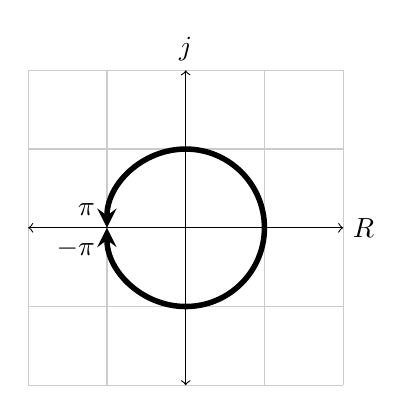
\begin{tikzpicture}
        \draw[thin,gray!40] (-2,-2) grid (2,2);
        \draw[<->] (-2,0)--(2,0) node[right] {$R$};
        \draw[<->] (0,-2)--(0,2) node[above]{$j$};
        \draw[line width=2pt,black,-stealth] (1,0) arc (0:180:1) node [anchor=south east]{$\pi$};
        \draw[line width=2pt,black,-stealth] (1,0) arc (0:-180:1) node [anchor=north east]{$-\pi$};
    \end{tikzpicture}
    \caption{Intervalo del argumento}